%! Author = Miszka and Tamarka
%! Date = 10.03.2022

% Preamble
\documentclass[11pt]{amsart}

% Packages
\usepackage{float}
\usepackage[T1]{fontenc}
\usepackage{geometry}
\usepackage{parskip}
\usepackage{amsmath}
\usepackage{amsfonts}
\usepackage{amsthm}
\usepackage{amssymb}
\usepackage{titling}
%\usepackage{itemize}
\usepackage{enumerate}
\usepackage{multirow}
\usepackage{graphics}
\usepackage{graphicx}
\usepackage{caption}
\usepackage{array}
\usepackage{xcolor}

\graphicspath{ {./fig/} }


%\setlength{\droptitle}{-2cm}
%\newgeometry{tmargin=1.9cm, bmargin=1.9cm, lmargin=1.7cm, rmargin=1.7cm}

\DeclareMathOperator*{\argmin}{arg\,min}

\newcommand{\tami}[1]{{\textcolor{magenta}{#1}}}
\newcommand{\domi}[1]{{\textcolor{green}{#1}}}

\author{Tamara Frączek, Dominik Mika}
\title{Methods of classification and dimensionality reduction - Report 1}
\date{\today}

% Document
\begin{document}
\maketitle


\section{Introduction}

\subsection*{Statement of the problem}

In this task we have to create a movie recommender system for our users.
\domi{We have users who rated some movies}.
Of course, not every user rated every movie and it is our task to fill those gaps.
So if one user hasn't seen one movie, we want to predict how he would like it.



%some movies and some information about how our users rate our movies.
%Since, of course, not every user rated every movie, we want to predict how they would like the movies from our list.

%We have the data containing information how users rate some movies.
%Our task is to create a recommender system, so having only some data we want to predict all ratings.

For this purpose we build few algorithms using different methods of predicting.
%These methods are described in ...
Of course different methods will give us different results (errors).
Our task is to tune parameters of those methods and try to get the best possible ratings prediction.



\subsection*{Description of methods}

In this problem, we use different methods which are subset of PCA methods. They are often used for dimensionality reduction and matrix factorization.

\subsubsection*{SVD1}

This method gets a $n \times d$ dimensional matrix $Z$ and approximate it by a different matrix $\tilde{Z}$.
Since we want somehow $\tilde{Z}$ to maintain only ''the most important'' information from $Z$, then the rank of $\tilde{Z}$ is to be much smaller than rank of $Z$.
Precisely, we want to find matrix $\tilde{Z}_r$ of rank $r$ ($r < rank(Z)$ and $r$ is a parameter), so that $\|Z - \tilde{Z}_r\|$ is small.

Using SVD decomposition $Z = U \Lambda^{\frac{1}{2}} V^T$ we construct $\tilde{Z}$ as
\[\tilde{Z}_r = U_r \Lambda_r^{\frac{1}{2}}V_r^T,\]
where $\Lambda_r$ contains $r$ biggest eigenvalues of $Z$ and $U_r$, $V_r$ contains only columns corresponding to those eigenvalues.

\subsubsection*{SVD2}

It is an iterative method.
We perform SVD1 on matrix $Z$, then on the result of first SVD1 and so on.
The algorithm can be stopped after a fixed number of iterations or some stop condition can be established.


\subsubsection*{NMF}

Similarly as in SVD1 the method obtain a $n \times d$ dimensional matrix $Z$ and approximate it by $\tilde{Z}$.
This time $\tilde{Z}$ is constructed as $\tilde{Z}_r = W_r H_r $, where $W_r$ and $H_r$ are matrices with non-negative elements ($W_r$ has $r$ columns and $H_r$ has $r$ rows).
Precisely, we look for such $W_r$ and $H_r$ that $\|Z - W_r H_r \|^2$ is the smallest, where $\|A\|^2 = \sum_{i, j} A_{ij}^2$.

\subsubsection*{SGD}


\section{Implementation}

\subsection*{Description of the data}

Our data contains information 100837 ratings - exactly 610 users rated 9724 movies.
The columns are: \textsf{userId} (integer), \textsf{movieId} (integer) and \textsf{rating} (integer), where \textsf{userId} is a unique user id and \textsf{movieId} is a unique movie id.


We keep this data in two-dimensional matrix of size $n \times d$ where $n$ is the number of users and $d$ is the number of movies.
In element $(i,j)$ we put the rate of the user $i$ of the movie $j$.
If the user $i$ haven't rated the movie $j$ we leave the element empty.


\subsection*{Performing methods}

\tami{??tutaj jakaś intuicja po co dzielić dane??}

So to be able to evaluate the quality of the programs we split our data to two parts: train set and test set.
The train set is used to build the programs.
And the test set is used to evaluate how our programs work.


To give our programs enough information about every user we split the data so that the train set contain 90\% of ratings of each user (and the test set the remaining ones).


Let call the matrix containing the data from the train set as $\boldsymbol{Z}$ and the matrix containing the data from the test set as $\boldsymbol{T}$.


\subsection*{Quality of the system}

Assume that our algorithm return a matrix $\boldsymbol{Z}^{'}$.
Then the quality of our programs is computed as \textbf{root-mean square error}
\[\textsf{RMSE} =
\sqrt{\frac{1}{|\mathcal{T}|} \sum_{(u,m) \in \mathcal{T}} \left(\boldsymbol{Z}^{'}[u,m] - \boldsymbol{T}[u,m] \right)^2}\]
where $\mathcal{T}$ contains pairs $(u,m)$ from test set.


\subsection*{Imputing the missing data}

Because three of our methods (SVD1, SVD2 and NMF) are given a full matrix $\boldsymbol{Z}$, so they need the missing data to be imputed before performing.

We decided to impute the data in 4 different ways:
\begin{itemize}
    \item putting 0 everywhere,
    \item putting global mean everywhere,
    \item putting row mean,
    \item putting weighted row and column mean ($\alpha \cdot \text{\textsf{row\_mean}} + (1-\alpha) \cdot \text{\textsf{col\_mean}}$, where $\alpha$ is \tami{...}).
\end{itemize}

\begin{figure}[H]
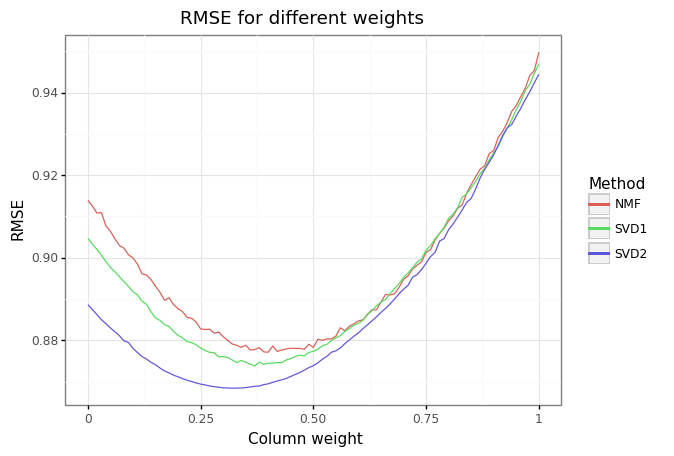
\includegraphics[scale=0.6]{weights}
\label{fig:figure}
\end{figure}

\tami{??In SVD2 we make a correction -- czy to tu}

\tami{tutaj przemyślenia na temat tego czemu niektóre metody działają lepiej i dlaczego}

\subsection*{Choosing parameters}

\subsubsection*{SVD1} r
\begin{figure}[H]
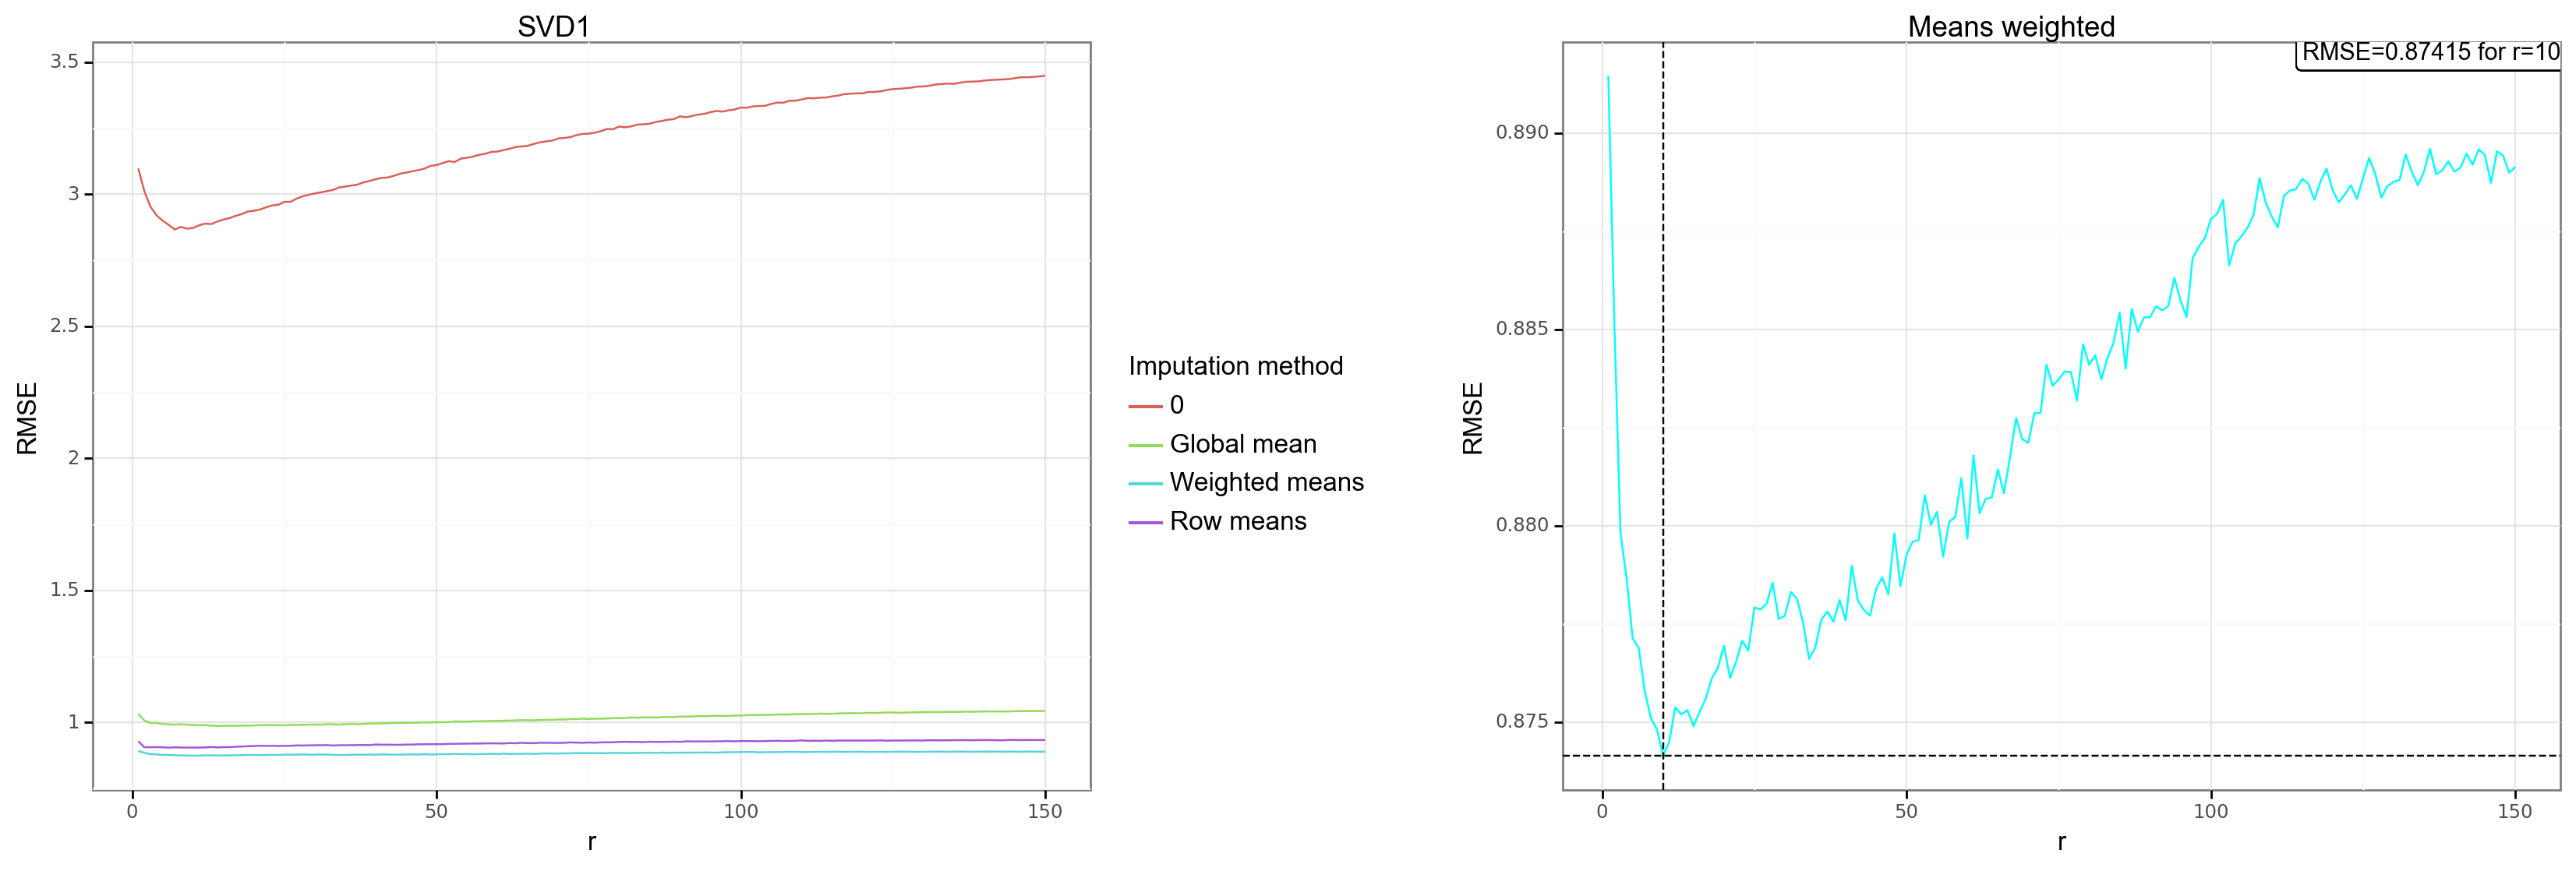
\includegraphics[scale=0.45]{svd1_all}
\label{fig:figure}
\end{figure}
\tami{te wykresy po lewej trzeba zrobić od 0}

\subsubsection*{SVD2} r, czy tutaj \tami{warunek zatrzymania ????????}
\begin{figure}[H]
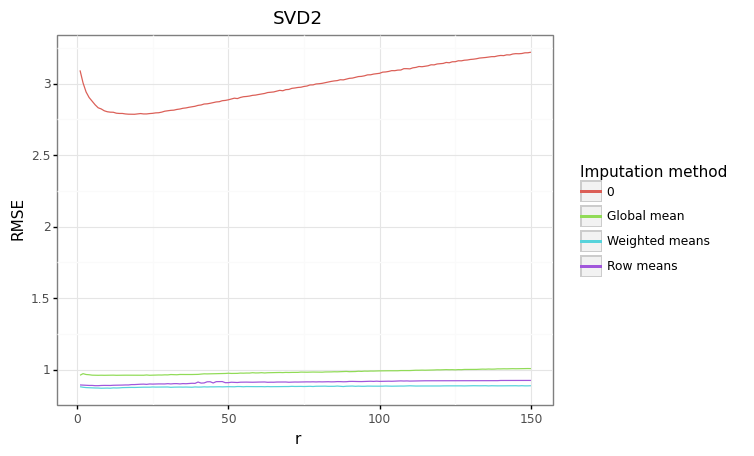
\includegraphics[scale=0.45]{svd2_all}
\label{fig:figure}
\end{figure}

\subsubsection*{NMF} r
\begin{figure}[H]
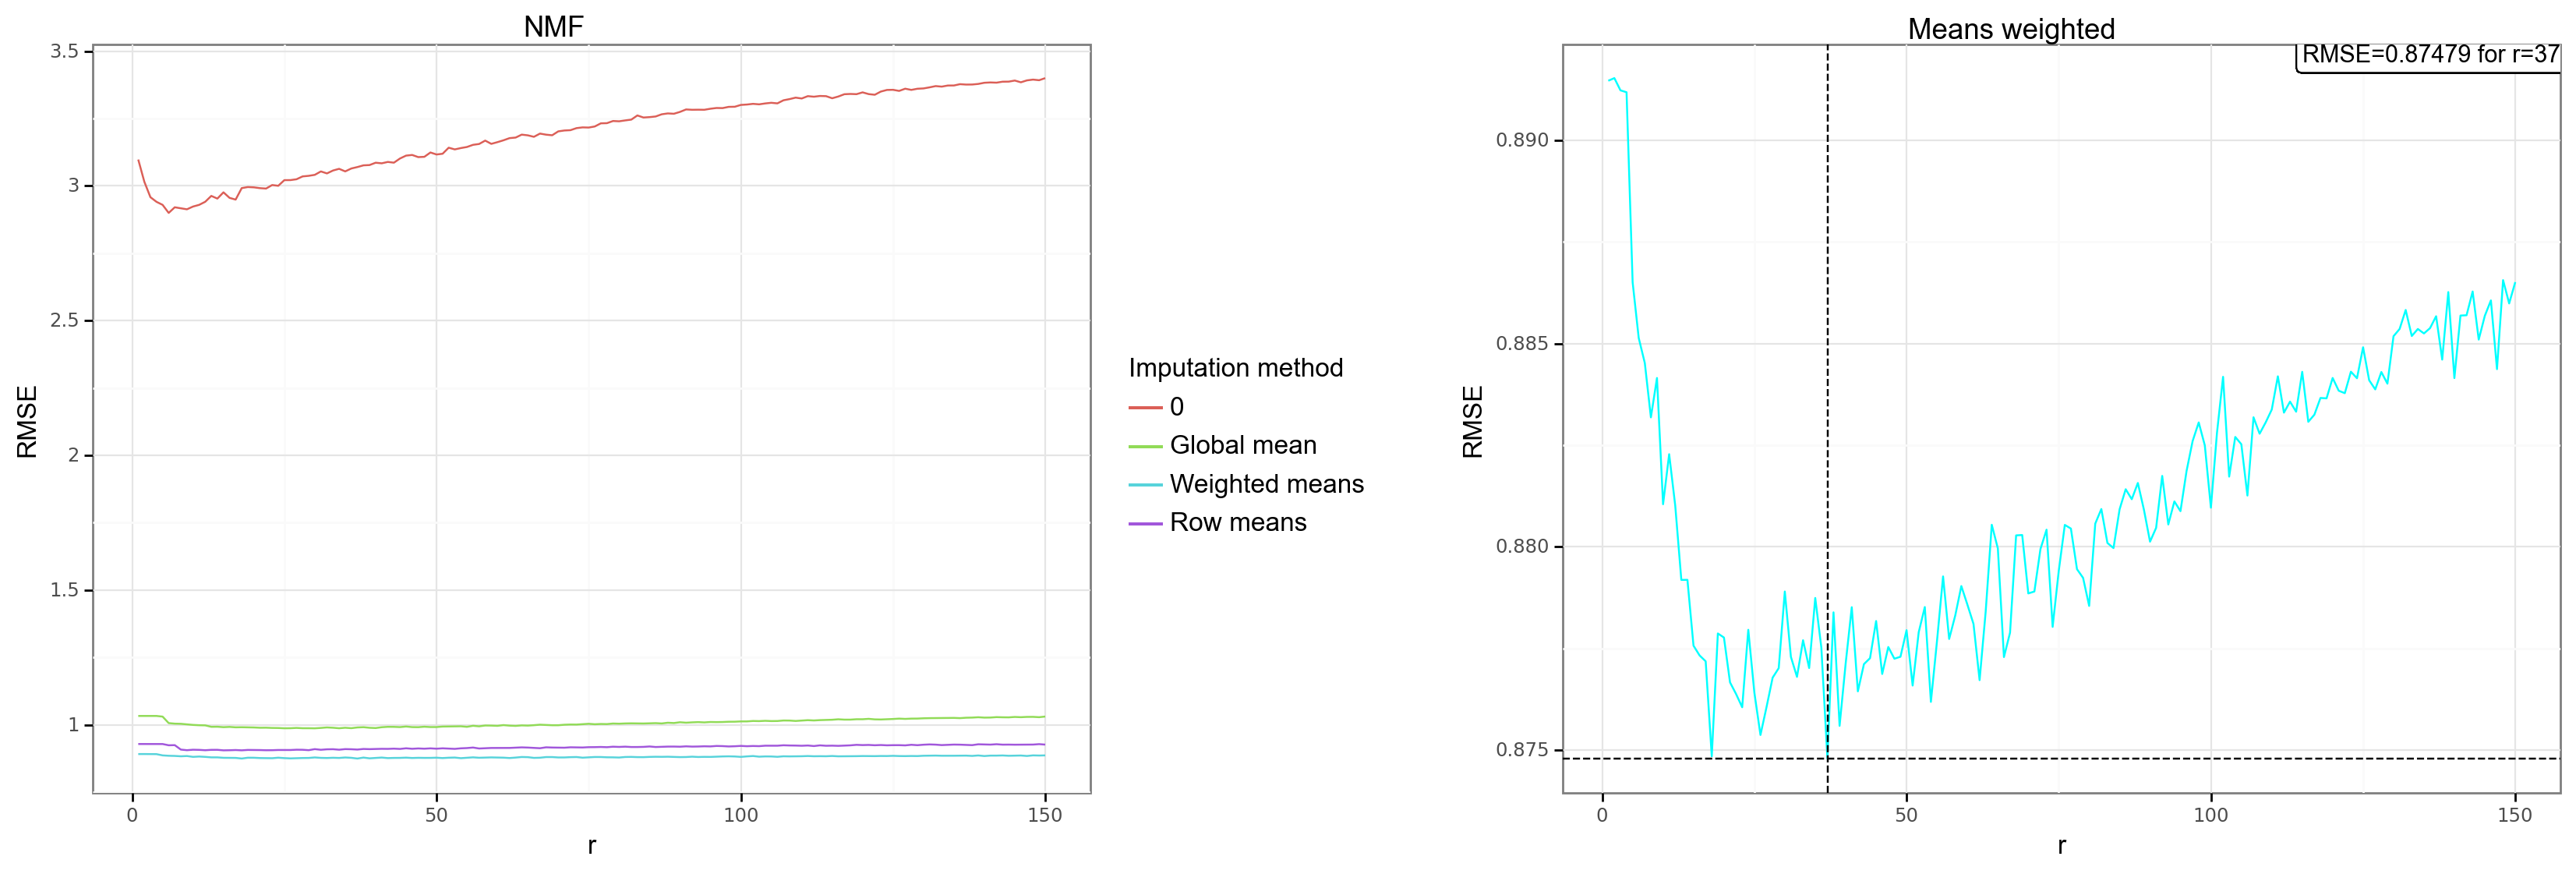
\includegraphics[scale=0.45]{nmf_all}
\label{fig:figure}
\end{figure}



\begin{figure}[H]
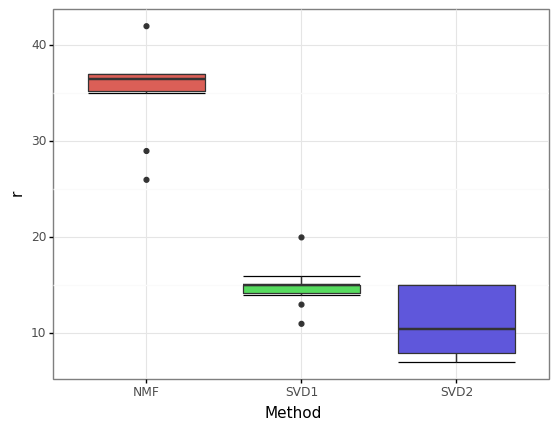
\includegraphics[scale=0.6]{boxplot_reps}
\label{fig:figure}
\end{figure}

\subsubsection*{SGD} $\eta$, warunek początkowy

\section{Results}



\end{document}